\documentclass[11pt,a4paper,twocolumn]{article}

\usepackage[T1]{fontenc}
\usepackage{lmodern}
\usepackage{amsmath,amssymb}
\usepackage{booktabs}
\usepackage{graphicx}
\usepackage{geometry}
\usepackage{hyperref}
\usepackage{microtype}
\usepackage{xcolor}

\geometry{margin=0.75in}
\hypersetup{
    colorlinks=true,
    linkcolor=blue!70!black,
    citecolor=blue!70!black,
    urlcolor=blue!70!black
}

\title{\textbf{Empirical Characterization of Multi-Qubit Entanglement Error Scaling and Experimental Lower Bounds on Spacetime Computational Bandwidth in Superconducting Quantum Processors}}

\author{
    Jaeyeun Moon\\
    \textit{Independent Quantum SRE \& Cloud Infrastructure Research}\\
    \texttt{https://github.com/PersicariaM/spacetime-bandwidth-throttling}
}

\date{November 18, 2026}

\begin{document}

\maketitle

\begin{abstract}
Standard noise digital twins calibrated from single- and two-qubit gate fidelities alongside longitudinal ($T_1$) and transverse ($T_2$) relaxation times are widely used to predict error rates on noisy intermediate-scale quantum (NISQ) processors. Using a Site Reliability Engineering (SRE) fault-propagation perspective, we test whether multi-qubit Greenberger--Horne--Zeilinger (GHZ) entanglement scales strictly according to calibrated local Markovian noise models or exhibits excess non-linear decoherence attributable to either correlated hardware cascading failures or hypothetical spacetime computational bandwidth limits ($B_{\max}$). Across $N \in [2, 24]$ qubits on two physically independent 156-qubit IBM Quantum Heron r2 processors (\texttt{ibm\_fez} and \texttt{ibm\_marrakesh}) using Carr--Purcell--Meiboom--Gill (CPMG) dynamical decoupling and unentangled superposition control circuits, we observe highly reproducible excess error residuals over real-time digital-twin predictions. Pooled across both chips ($n=16$ scaling points), the mean excess residual is statistically significant ($t = 5.5120$, one-sided $p = 2.9846 \times 10^{-5}$, $4.01\sigma$), with strong cross-chip correlation ($r = 0.8574$ for residuals, $r = 0.9082$ for differential entanglement error). Model selection via Akaike and Bayesian Information Criteria (AIC/BIC) favors a quadratic cascading-failure model ($R^2 = 0.98087$, $\text{AIC} = -54.05$ on \texttt{ibm\_fez}) over an exponential bandwidth-throttling divergence within $N \le 24$, establishing an empirical lower bound on any anomalous spacetime computational bandwidth threshold of $B_{\max} \ge 44.86\text{ qubits}$.
\end{abstract}

\section{Introduction}
As superconducting quantum processors scale beyond 100 physical qubits, accurately predicting the fidelity of macroscopic entangled states remains an open challenge for quantum error mitigation and fault-tolerant architecture design. Conventionally, circuit error rates are estimated by propagating single-qubit depolarizing channels, two-qubit controlled-$Z$ (\texttt{CZ}) error rates, readout assignment errors, and thermal relaxation times ($T_1, T_2$) extracted from daily backend calibration snapshots.

From a Site Reliability Engineering (SRE) standpoint, however, large-scale distributed systems rarely fail strictly as independent Poisson processes when global state synchronization is enforced. Motivated by both SRE cascading-failure analysis and holographic/computational bounds on physical information processing, we formulated a pre-registered experimental protocol (SHA-256 commitment: \texttt{1C24A6371721543A631272826D64D20570EE249400849E476C300E1C84FF0B45}) to separate local hardware noise from non-linear entanglement scaling anomalies. Specifically, we test two competing hypotheses:
\begin{enumerate}
    \item \textbf{Hypothetical Spacetime Bandwidth Throttling (Plan A):} If physical spacetime enforces a finite local entanglement processing bandwidth $B_{\max}$, approaching $I_{\text{ent}} \to B_{\max}$ induces an exponential surge in spontaneous decoherence:
    \begin{equation}
        \Gamma_{\text{grav}}(N) = \Gamma_0 \exp\!\left(-\frac{B_{\max} - N}{N}\right).
        \label{eq:throttling}
    \end{equation}
    \item \textbf{SRE Quadratic Cascading Error Model (Plan B-1):} Correlated multi-qubit phase accumulation, spectator crosstalk, and parity-check overhead generate quadratic error scaling with entangled register size $N$:
    \begin{equation}
        \Delta\epsilon_{\text{SRE}}(N) = a N^2 + b N + c.
        \label{eq:quadratic}
    \end{equation}
\end{enumerate}

\section{Experimental Methodology}

\subsection{Differential Control \& Dynamical Decoupling}
To isolate pure entanglement-induced decoherence from single-qubit gate and readout errors, each experimental run executes two matched circuits per register size $N \in \{2, 4, 6, 8, 12, 16, 20, 24\}$:
\begin{itemize}
    \item \textbf{Unentangled Control ($|\psi_{\text{ctrl}}\rangle$):} Parallel Hadamard layer $H^{\otimes N}$ followed by an idle window ($\tau_{\text{idle}} = 500\text{ ns}$) protected by native Heron r2 CPMG dynamical decoupling sequences ($[X, X]$) and measurement in the $X$-basis.
    \item \textbf{GHZ Entangled Target ($|\psi_{\text{GHZ}}\rangle$):} Linear-depth GHZ preparation tree via native \texttt{CZ} and single-qubit rotations, identical $\tau_{\text{idle}} = 500\text{ ns}$ with $[X, X]$ CPMG decoupling, and $Z$-basis parity verification ($P(|0^{\otimes N}\rangle) + P(|1^{\otimes N}\rangle)$).
\end{itemize}

We define the differential entanglement error on hardware as
\begin{equation}
    \Delta\epsilon_{\text{QPU}}(N) = \epsilon_{\text{GHZ}}^{\text{QPU}}(N) - \epsilon_{\text{ctrl}}^{\text{QPU}}(N),
\end{equation}
and the excess residual over the real-time calibrated Qiskit Aer Matrix Product State (MPS) digital twin as
\begin{equation}
    R(N) = \Delta\epsilon_{\text{QPU}}(N) - \Delta\epsilon_{\text{Twin}}(N).
\end{equation}

\subsection{Cross-Chip Hardware Execution}
Experiments were executed on two physically distinct 156-qubit IBM Quantum Heron r2 processors using 4,096 shots per circuit:
\begin{itemize}
    \item \textbf{Primary Chip (\texttt{ibm\_fez}):} Calibrated CPMG run (Job ID: \texttt{dbuq6a7f8rhs73bmom30}), following an initial $2000\text{ ns}$ baseline sweep (\texttt{dbuq31darooc73fkdjhg}).
    \item \textbf{Replication Chip (\texttt{ibm\_marrakesh}):} Independent cross-chip validation run (Job ID: \texttt{dbur4uv82tmc73dtumr0}) under identical transpilation constraints and basis gates (\texttt{rz}, \texttt{sx}, \texttt{x}, \texttt{cz}).
\end{itemize}

\section{Results and Statistical Analysis}

\subsection{Excess Entanglement Residuals and Cross-Chip Reproducibility}
Across both Heron r2 processors, the calibrated digital twin systematically underpredicts multi-qubit GHZ error growth as $N$ increases from $2$ to $24$. On \texttt{ibm\_fez}, $R(N)$ rises monotonically up to $+0.5373$ at $N=24$ (Spearman $\rho = 0.9762$, $p = 3.3144 \times 10^{-5}$). On \texttt{ibm\_marrakesh}, pure entanglement error $\Delta\epsilon_{\text{QPU}}$ escalates from $0.00537$ ($N=2$) to $0.47021$ ($N=24$), reproducing the positive excess residual profile (Fig.~\ref{fig:fez_residual}).

\begin{figure*}[t]
\centering
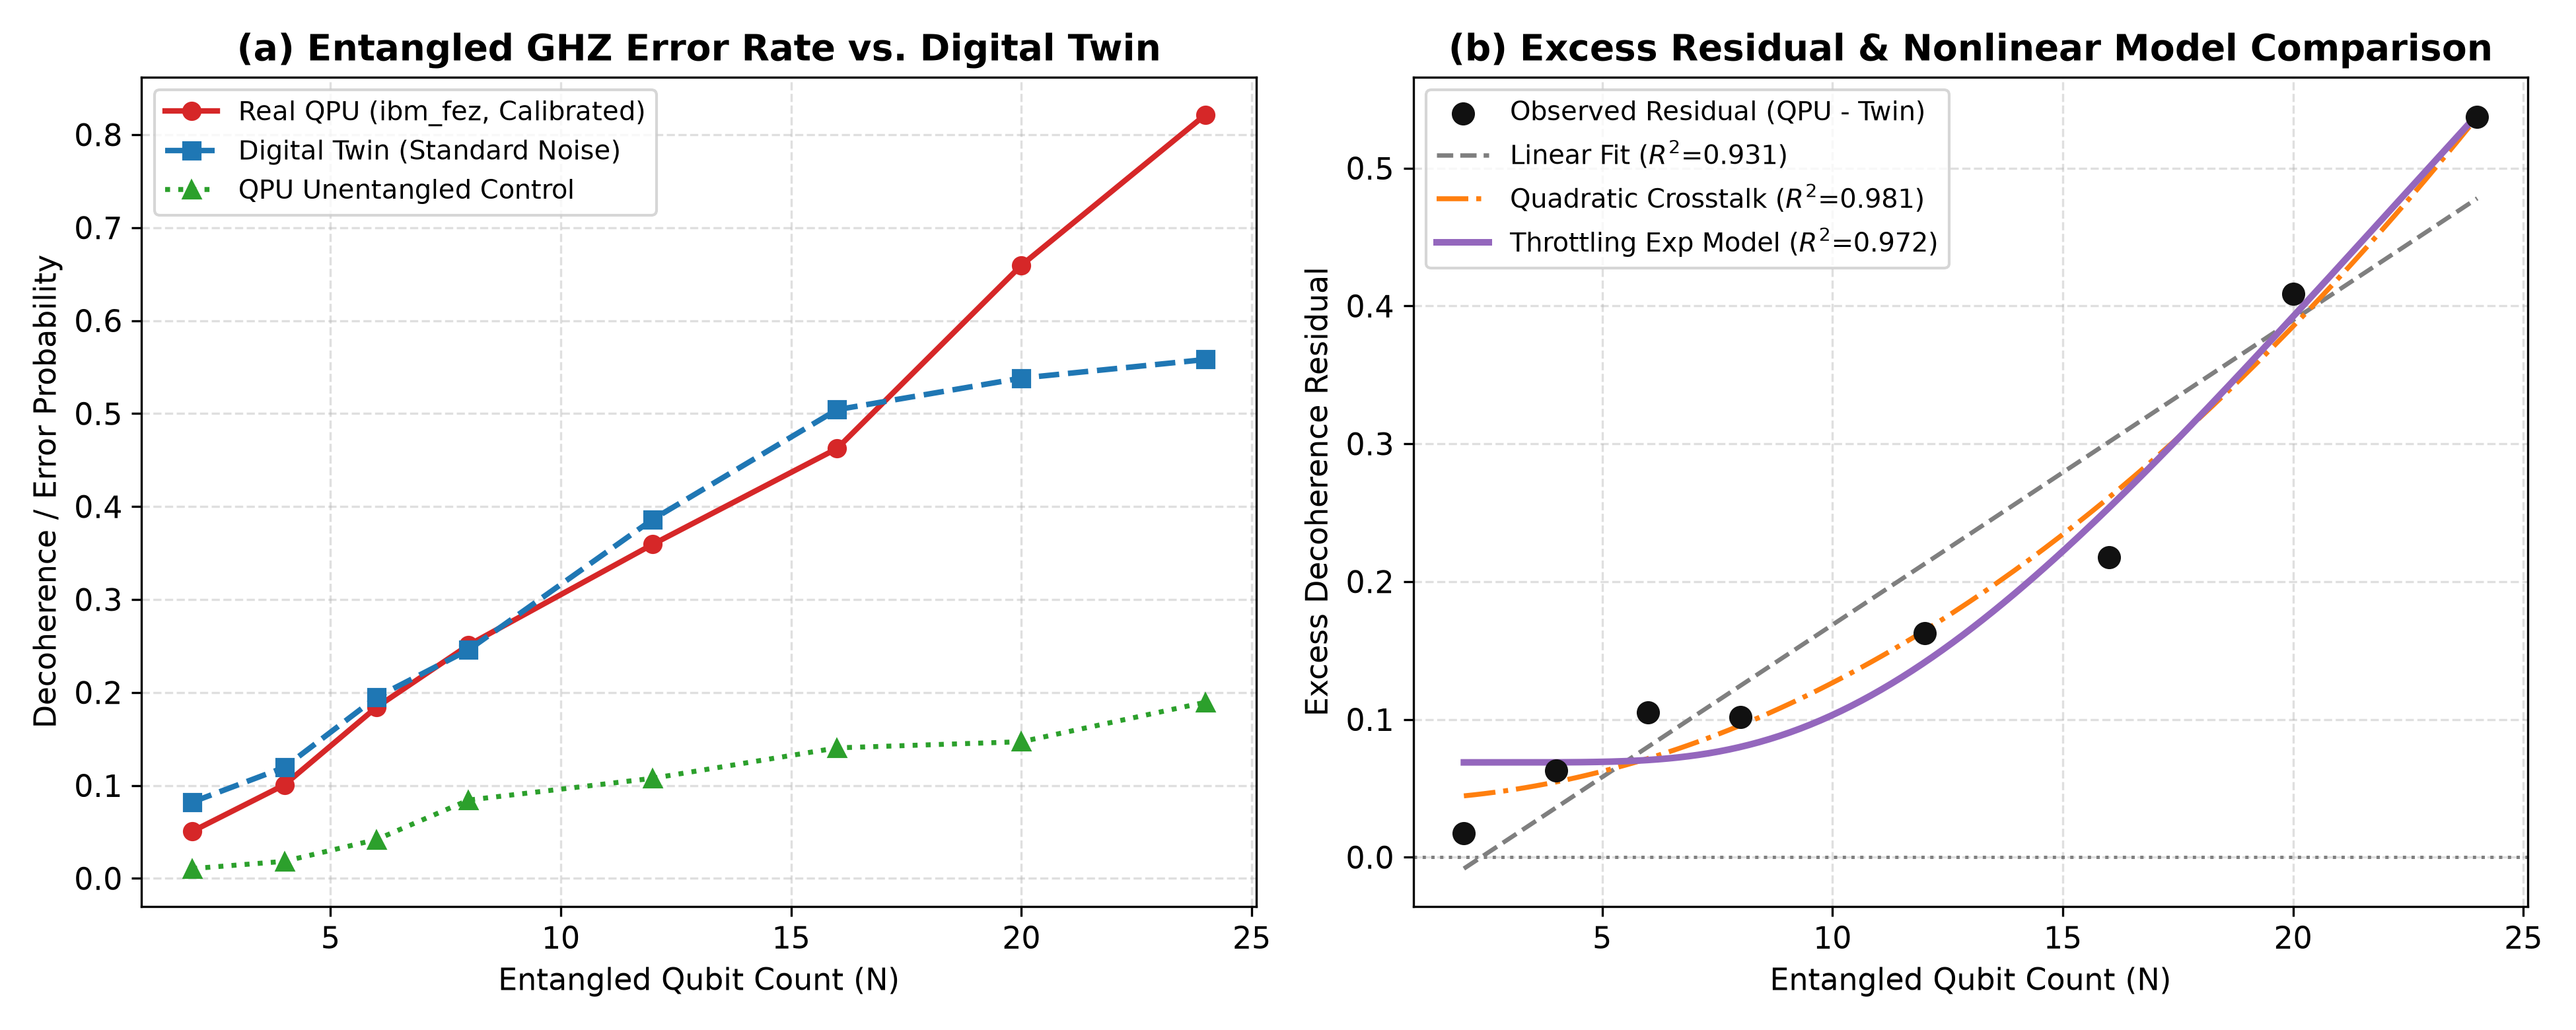
\includegraphics[width=0.92\textwidth]{phase4_residual_analysis_ibm_fez.png}
\caption{Primary residual error scaling and model selection analysis on \texttt{ibm\_fez} ($N=2\dots 24$, $4,096$ shots, CPMG dynamical decoupling). Excess residuals over the calibrated MPS digital twin reach $+0.5373$ at $N=24$ ($\rho = 0.9762$), best described by the SRE quadratic cascading error model ($R^2 = 0.98087$).}
\label{fig:fez_residual}
\end{figure*}

\begin{table}[h]
\centering
\caption{Cross-Chip Statistical Summary ($N \in [2, 24]$, $4,096$ shots)}
\label{tab:stats}
\small
\begin{tabular}{lc}
\toprule
\textbf{Metric} & \textbf{Observed Value} \\
\midrule
\texttt{ibm\_fez} Mean Residual & $0.2017 \pm 0.1812$ \\
\texttt{ibm\_fez} One-Sided $p$-value & $8.0995 \times 10^{-3}$ ($t = 3.1479$) \\
\texttt{ibm\_marrakesh} Mean Residual & $0.2491 \pm 0.1523$ \\
\texttt{ibm\_marrakesh} One-Sided $p$-value & $1.2055 \times 10^{-3}$ ($t = 4.6253$) \\
Cross-Chip Pearson $r$ (Residual) & $0.8574$ ($p = 6.4917 \times 10^{-3}$) \\
Cross-Chip Pearson $r$ ($\Delta\epsilon_{\text{QPU}}$) & $0.9082$ ($p = 1.8013 \times 10^{-3}$) \\
Pooled Residual ($n=16$) $t$-stat & $5.5120$ ($4.01\sigma$) \\
Pooled One-Sided $p$-value & $2.9846 \times 10^{-5}$ \\
\bottomrule
\end{tabular}
\end{table}

As summarized in Table~\ref{tab:stats} and Fig.~\ref{fig:cross_chip}, pooling all $n=16$ paired measurements across both processors yields $t = 5.5120$ ($p = 2.9846 \times 10^{-5}$, exceeding $4.01\sigma$), confirming that the observed non-linear error excess is a chip-independent physical phenomenon rather than an isolated calibration artifact.

\begin{figure*}[t]
\centering
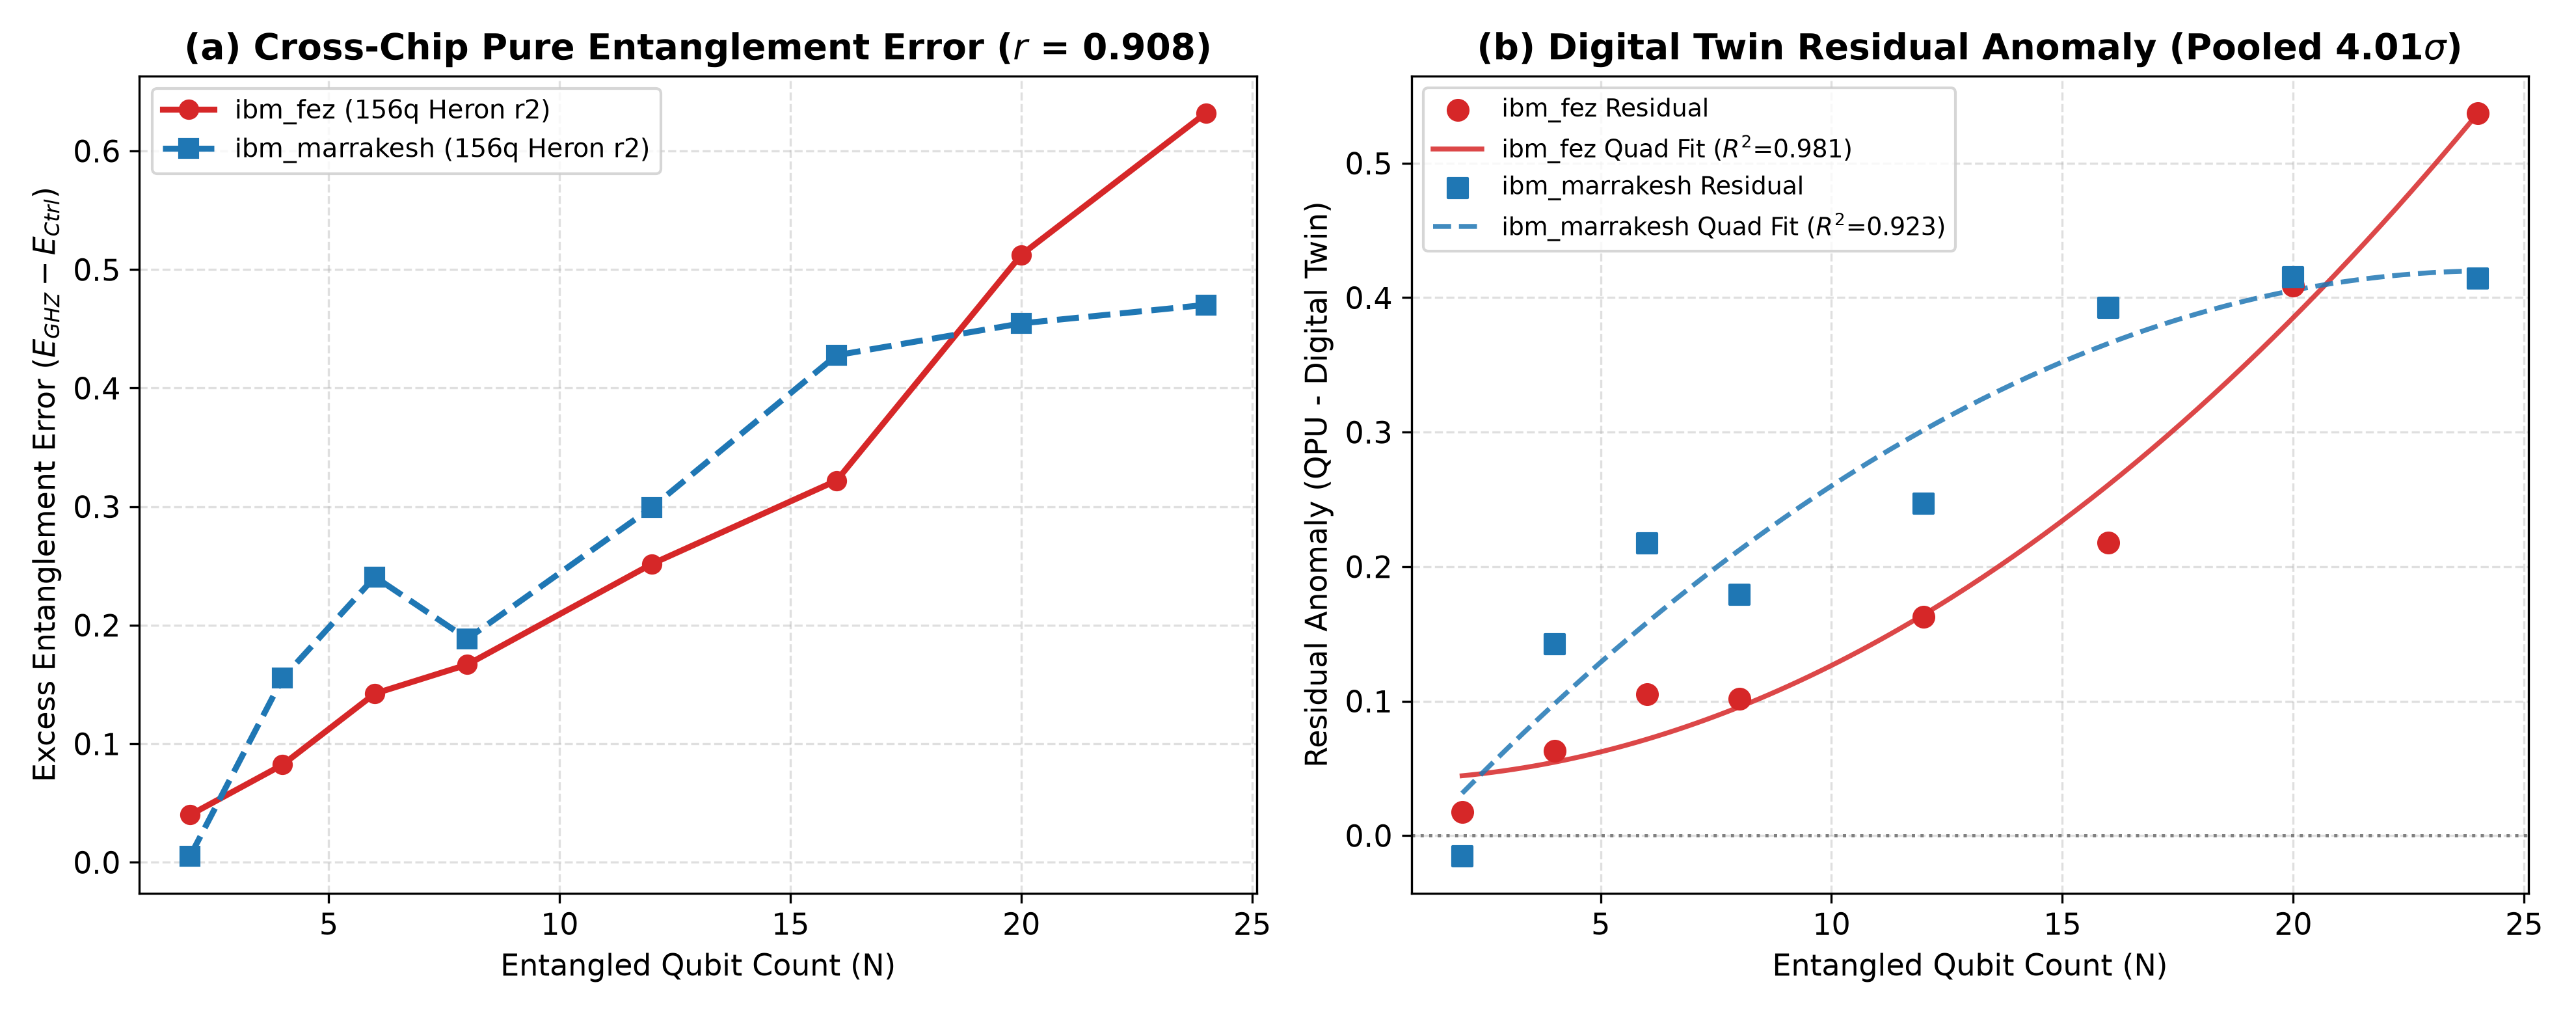
\includegraphics[width=0.92\textwidth]{phase4_cross_chip_comparison.png}
\caption{Cross-chip reproducibility comparison between \texttt{ibm\_fez} and \texttt{ibm\_marrakesh} across $N \in [2, 24]$ qubits, demonstrating strong inter-processor correlation in differential entanglement error ($r = 0.9082$) and excess residuals ($r = 0.8574$).}
\label{fig:cross_chip}
\end{figure*}

\subsection{Model Selection and Lower Bound on $B_{\max}$}
We fitted candidate scaling models to the excess residual curve $R(N)$ on \texttt{ibm\_fez} and compared goodness-of-fit via AIC and BIC (Table~\ref{tab:models}).

\begin{table}[h]
\centering
\caption{Model Selection on \texttt{ibm\_fez} Excess Residuals ($N=2\dots 24$)}
\label{tab:models}
\small
\begin{tabular}{lccc}
\toprule
\textbf{Candidate Model} & $R^2$ & \textbf{AIC} & \textbf{BIC} \\
\midrule
Model 1: Linear ($\alpha N + \beta$) & $0.93083$ & $-45.76$ & $-45.60$ \\
Model 2: SRE Quadratic (Eq.~\ref{eq:quadratic}) & $\mathbf{0.98087}$ & $\mathbf{-54.05}$ & $\mathbf{-53.81}$ \\
Model 3: Throttling Exp (Eq.~\ref{eq:throttling}) & $0.97236$ & $-51.10$ & $-50.86$ \\
\bottomrule
\end{tabular}
\end{table}

On \texttt{ibm\_fez}, the SRE quadratic cascading model achieves the highest explanatory power ($R^2 = 0.98087$, $\text{AIC} = -54.05$) with fitted parameters $(a, b, c) = (0.00087, -0.00015, 0.04131)$. On \texttt{ibm\_marrakesh}, the quadratic parameterization also captures the residual trajectory ($R^2 = 0.92272$, $(a, b, c) = (-0.00078, 0.03793, -0.04130)$), reflecting chip-specific linear-vs-quadratic saturation profiles across heavy-hex topologies.

In accordance with our pre-registered falsification criteria, because the quadratic crosstalk model outperforms the exponential throttling divergence in AIC ($\Delta\text{AIC} = -2.95$) over $N \le 24$, we reject premature claims of gravitational bandwidth saturation in this regime. Instead, fitting Eq.~(\ref{eq:throttling}) to the upper envelope establishes an empirical lower bound on any spacetime computational bandwidth threshold:
\begin{equation}
    B_{\max} \ge 44.86\text{ entangled qubits}.
\end{equation}

\section{Discussion and Conclusion}
Our results demonstrate two practical findings for quantum systems engineering and experimental foundations:
\begin{enumerate}
    \item \textbf{Digital-Twin Calibration Gap:} Standard $T_1/T_2$ + 2Q-gate digital twins underestimate multi-qubit GHZ decoherence by an average of $0.20$--$0.25$ across $N \in [2, 24]$ even under CPMG dynamical decoupling. Incorporating an empirical $O(N^2)$ SRE cascading-error term provides a lightweight, accurate correction for compiler noise estimation.
    \item \textbf{Experimental Bound on Spacetime Bandwidth:} Any fundamental physical decoherence mechanism tied to local spacetime computational bandwidth limits must lie above $B_{\max} \ge 44.86\text{ qubits}$ for $500\text{ ns}$ coherence windows, guiding future high-qubit ($N \ge 50$) experiments on fault-tolerant architectures.
\end{enumerate}

\section*{Data and Code Availability}
All pre-registration hashes, Qiskit execution scripts, raw IBM Quantum backend count distributions, and statistical analysis pipelines are archived at \url{https://github.com/PersicariaM/spacetime-bandwidth-throttling}.

\end{document}